% \pagebreak[4]
% \hspace*{1cm}
% \pagebreak[4]
% \hspace*{1cm}
% \pagebreak[4]

\chapter{Background and Model Selection}
\ifpdf
    \graphicspath{{Chapter1/Chapter1Figs/PNG/}{Chapter1/Chapter1Figs/PDF/}{Chapter1/Chapter1Figs/}}
\else
    \graphicspath{{Chapter1/Chapter1Figs/EPS/}{Chapter1/Chapter1Figs/}}
\fi

\section{Model Selection}
Our first task in implementing a sign recognition system was to determine a model suitable for the task of gesture recognition. We required a model which could be trained on a moderate sized training set and which is computationally efficient enough to be run in real time. Our research determined that Hidden Markov Models, Neural Networks or a Finite State Machine approach would be suitable for gesture recognition and that these models had been used for similar applications before~\citep{mitra2007gesture}. We decided that Hidden Markov Models would be the most suitable for the task of sign language recognition because they are approximately \emph{scale invariant}, meaning that they perform well even with minor scaling of their input, and hence resilient to the changes in input occurring when the signer changes.

\section{Hidden Markov Models}
A \emph{Hidden Markov Model} (HMM) is (following the definitions in~\cite{rabiner1989tutorial}) a doubly stochastic process which consists of an underlying discrete Markov chain with state set $S = \{S_1, \dots, S_n \}$ and stochastic matrix $A=[a_{i,j}]_{N\times N}$ where 
\begin{equation*}
a_{i,j} = \mathbb{P}(q_{t+1} = S_i | q_t = S_j) \text{  for each  } 1 \leq i,j \leq N
\end{equation*}
which is hidden from an observer in the sense that one cannot directly observe the current state of the Markov chain. Instead we have a collection of $M$ observable symbols, say $V = \{ v_1, \dots, v_M\}$, which may be observed with probability dependent on the state of the underlying Markov chain (Figure:~\ref{fig:hmmex}). We encode these so-called \emph{emission probabilities} in a matrix $B = [b_j(k)]_{N\times M}$ where
\begin{equation*}
b_j(k) = \mathbb{P}[v_k \text{ occurs at time }t | q_t = S_j] 
\end{equation*}
Now if we take an initial state distribution $\bm{\pi} = [\pi_1, \dots, \pi_N]$ for our Markov chain with
\begin{equation*}
\pi_i= \mathbb{P}[q_1 = S_i]
\end{equation*}
then the HMM generates a sequence of observations
\begin{equation*}
\bm{O} = O_1, O_2, \ldots , O_T
\end{equation*}
by the following process:
\begin{enumerate}
\item Choose an initial state $q_1 = S_i$ stochastically from the initial state distribution $\bm{\pi}$
\item For $t=1$ to $T$
\begin{enumerate}
\item[i.] Choose $O_t = v_k$ according to the distribution $b_i(k)$ of the current state $S_i$
\item[ii.] Stochastically transition to a new state $S_j$ from $S_i$ according to $A$ 
\end{enumerate}
\end{enumerate}

\begin{figure}[]
  \centering
    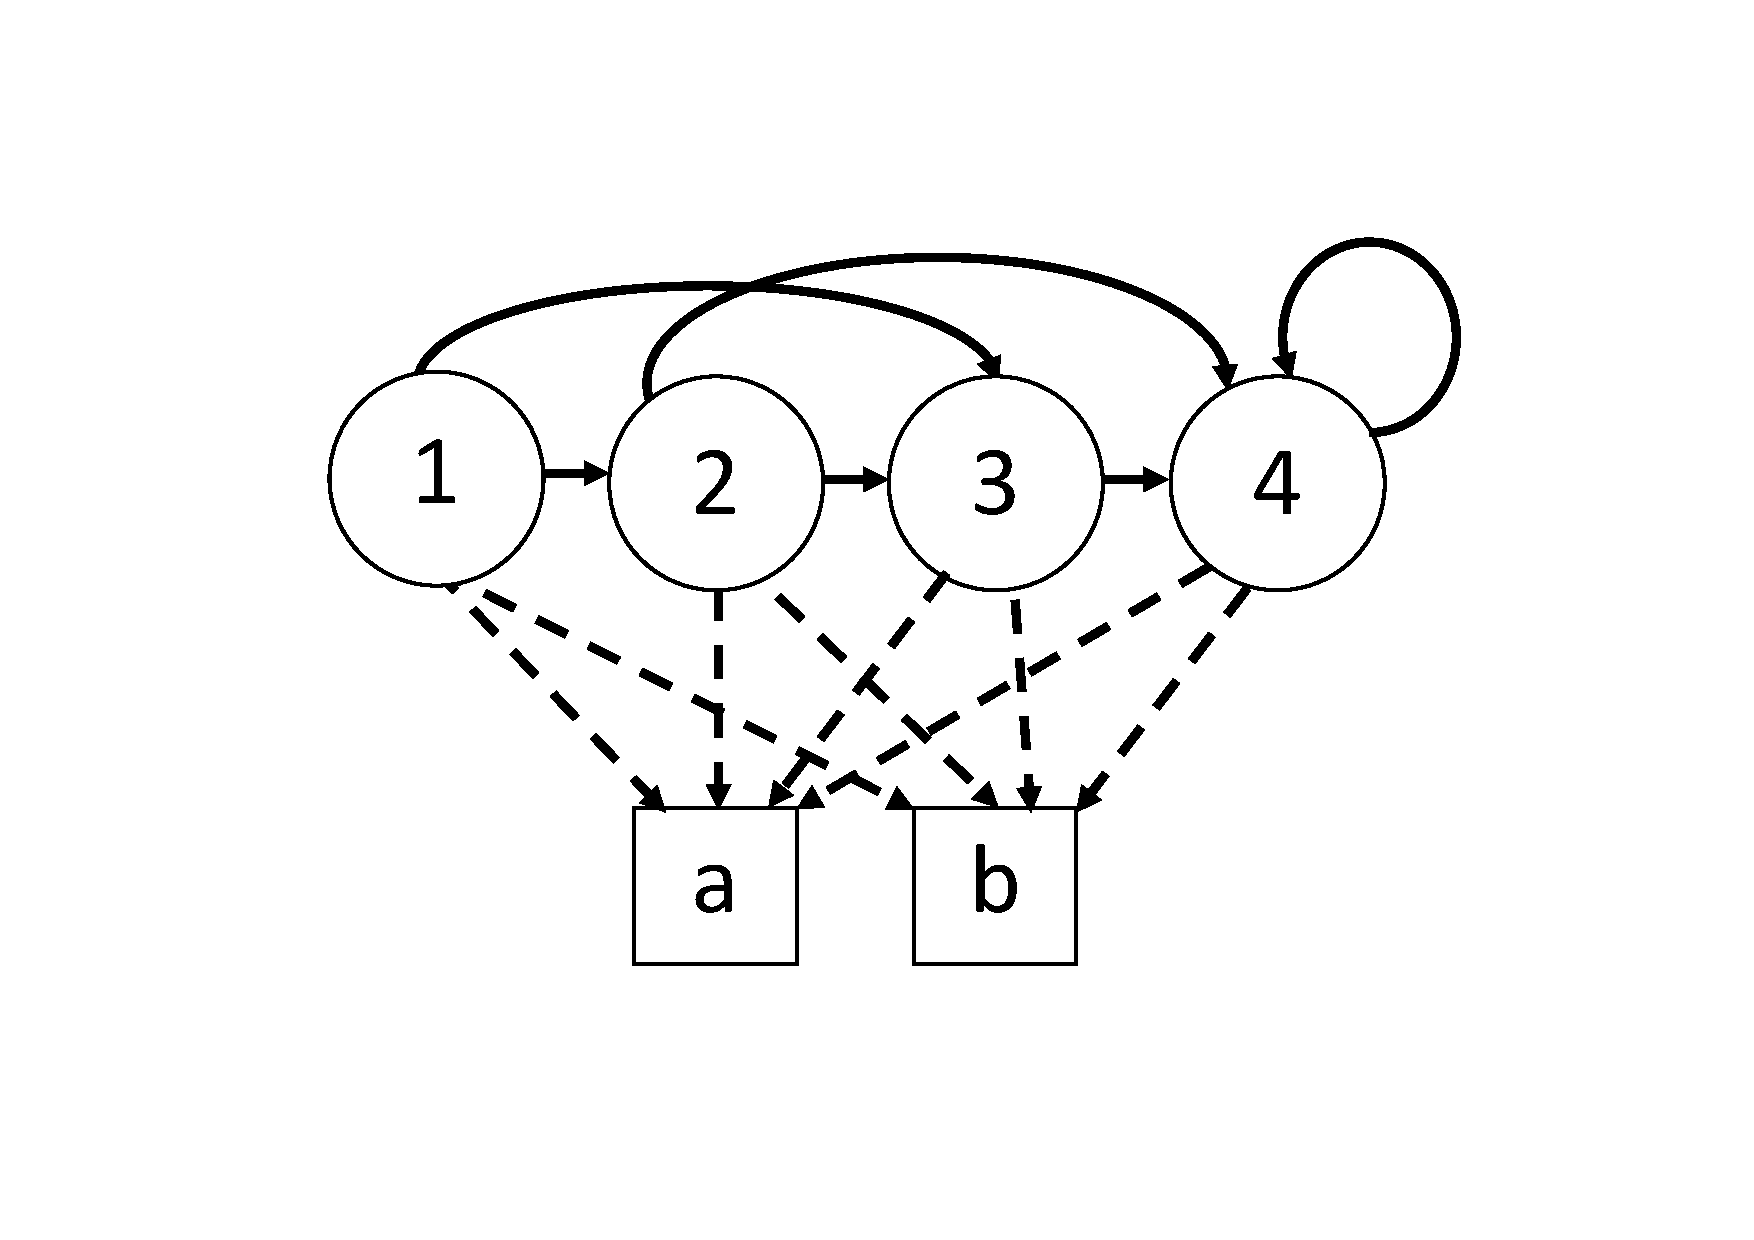
\includegraphics[width=0.7\textwidth]{ThesisFigs/HMMExample}
  \caption{A Hidden Markov Model. The underlying Markov Chain contains 4 states (depicted as circles) which emit two possible observations (a or b).}\label{fig:hmmex}
\end{figure}


Note now that a hidden Markov Model is entirely determined by the transition matrix $A$, the emissions matrix $B$ and the initial distribution $\bm{\pi}$ (the dimensions $N$ and $M$ are encoded in the dimensions of the matrices) hence for convenience we may denote a HMM by
\begin{equation*}
\lambda = (A,B, \bm{\pi})
\end{equation*}

Hidden Markov Models were first introduced by in a series of papers by L.E Baum and others in the late 1960s ~\citep{baum1966statistical,baum1970maximization} and have been since used to study handwriting recognition~\citep{bunke1995off}, speech recognition ~\citep{juang1991hidden, jelinek1998statistical}, natural language modelling~\citep{manning1999foundations, jurafsky2002speech} and biological processes ~\citep{krogh1994hidden, durbin1998biological, lio1998models}.
\\
\\
Given these definitions there exist three basic problems which form the basis of using HMMs as a tool for machine learning
\begin{enumerate}
\item Given an observation sequence $\bm{O} = O_1,O_2,\dots,O_T$ and a HMM $\lambda$, what is $\mathbb{P}(\bm{O}|\lambda)$ - the probability that the observation sequence $\bm{O}$ was produced by $\lambda$?
\item Given a HMM $\lambda$ and an observation sequence $\bm{O} = O_1,O_2,\dots,O_T $ what is the state sequence of the underlying Markov chain in $\lambda$ which is most likely to have generated $\bm{O}$?
\item Given an observation sequence $\bm{O}$, how to do we choose the parameters of $\lambda = (A,B,\bm{\pi})$ which best optimise $\mathbb{P}[\bm{O}|\lambda]$?
\end{enumerate}

In fact the problem of sign language gesture recognition can be seen as an instance of problems 3 and 1. First we take for each gesture $g$ a set of training data which are recordings of the joints in 3D space. This training data forms a collection of observation sequences $\bm{O}_1, \dots, \bm{O}_n$ which are used in a solution to problem 3 to parameterise a Hidden Markov Model $\lambda_g$ to model the gesture.

Then given a fresh observation sequence $\bm{O}$ we can use a solution to problem 1 to compute $\mathbb{P}[\bm{O} | \lambda_g]$ for each $g$. We can then take the gesture $g$ for which this probability is maximised and, provided the probability exceeds some threshold, conclude that the gesture $g$ corresponds to the observation sequence $\bm{O}$. 

\subsection{The Forward and Backward Variables}
Suppose we are given an observation sequence $\bm{O} = O_1,O_2,\dots,O_T$ and a HMM $\lambda$ and wish to solve the evaluation problem (problem 1). ~\citet{rabiner1989tutorial} notes that a direct computation of $\mathbb{P}[\bm{O}|\lambda]$ will take time order $\mathcal{O}(2TN^T)$ which is infeasible even for moderate values of $N$ and $T$. Instead we use a dynamic programming approach, \emph{the forward algorithm}, introduced in~\citet{baum1968growth} and ~\cite{baum1970maximization}.

Define the \emph{forward variables} $\alpha_t(i)$ for each $1\leq t \leq T$ and $1 \leq i \leq N$ by
\begin{equation*}
\alpha_t(i) = \mathbb{P}[O_1, \dots, O_t, q_t=S_i | \lambda]
\end{equation*}
These can be inductively computed by the following procedure 
\begin{align*}
&\alpha_1(i) = \pi_ib_i(O_1)\\
&\alpha_{t+1}(j) = \left[ \sum_{i=1}^{N} \alpha_{t}(i)a_{ij} \right]b_j(O_{t+1}) &\text{ for $1\leq t \leq T-1$ and $1 \leq j \leq N$}
\end{align*}
and further
\begin{align*}
\mathbb{P}[\bm{O} | \lambda] &= \sum_{i=1}^N \mathbb{P}[\bm{O}, q_T = S_i | \lambda] = \sum_{i=1}^N \alpha_T(i)
\end{align*}
The set of forward variables can be computed by dynamic programming in $\mathcal{O}(N^2T)$ time and hence we can compute $\mathbb{P}[\bm{O} | \lambda]$ in this time -  a significant improvement over direct computation.

Symmetrically to the forward variables we can define a collection of \emph{backward variables} by
\begin{equation*}
\beta_t(i) = \mathbb{P}[O_{t+1}, O_{t+2}, \dots, O_T | q_t = S_i, \lambda]
\end{equation*}
Which gives the probability of a partial observation sequence from a time $t$ given the state of the HMM $\lambda$ at time t. These too can be computed iteratively as
\begin{align*}
&\beta_T(i) = 1 &\text{ for each } 1 \leq i \leq N \\
&\beta_t(i)  = \sum_{j=1}^N a_{i,j}b_j(O_{t+1})\beta_{t+1}(j) &\text{ for } t = T-1, T-2,\dots,1 \text{ and } 1 \leq i \leq N \\
\end{align*}
and these too can be computed by dynamic programming in $\mathcal{O}(N^2T)$ time. The backward variables are not needed in the solution to the evalutation problem but are used in the following section to re-parameterise hidden Markov Models. 

\subsection{Forward-Backward Algorithm}
The problem of parameterising a Hidden Markov Model $\lambda$ is considerably more difficult than the other two problems of HMMs. In fact it is known that there is no analytic solution which provides a model $\lambda$ to maximise the probability of some observation sequence $\bm{O}$~\citep{rabiner1989tutorial}. Instead we must use local optimisation methods which given an initial parameterisation $\lambda_0$ iteratively improve it until $\mathbb{P}[\bm{O} | \lambda]$ reaches a local maximum. 

We will use a modified version of the \emph{Baum-Welch algorithm} introduced by~\citet{baum1970maximization} called the \emph{forward-backward algorithm}~\citep{rabiner1989tutorial} which is reproduced below. This algorithm is an instance of an expectation-maximization algorithm~\citep{moon1996expectation} which is a general technique used to determine maximum likelihood estimators in a number of machine learning models~\citep{bishop2006pattern}. \\
\\
For $t \in \{1, \dots, T-1\}$ and $i,j \in \{1, \dots, N\}$ define
\begin{equation*}
\gamma_t(i,j) = \mathbb{P}[q_t = S_i, q_{t+1}=S_j| \bm{O}, \lambda]
\end{equation*}
such that $\gamma_t(i,j)$ is the probability of being in state $S_i$ at time $t$ and transitioning to $S_j$ at the next time step given the HMM $\lambda$ and the observation sequence $\bm{O}$. Then by definiton of the foward and backward variables we have
\begin{align*}
\gamma_t(i,j) &= \frac{\alpha_t(i)a_{ij}b_j(O_{t+1})\beta(j)}{\mathbb{P}[\bm{O}|\lambda]}	
\end{align*}
We can define for each $1 \leq t \leq T-1$ and each $1 \leq i \leq N$ the probability of being in state $i$ at time $t$ by
\begin{equation*}
\gamma_t(i) = \mathbb{P}[q_t = S_n | \bm{O}, \lambda] = \frac{\alpha_t(i)\beta_t(i)}{\mathbb{P}[\bm{O}|\lambda]}
\end{equation*}
and then we have
\begin{equation*}
\gamma_t(i) = \sum_{j=1}^N \gamma_t(i,j)
\end{equation*}
Now using these equations we can compute
\begin{align*}
&\sum_{t=1}^{T-1} \gamma_t(i) = \text{The expected number of transitions from $S_i$} \\
&\sum_{t=1}^{T-1} \gamma_t(i,j) =  \text{The expected number of transitions from $S_i$ to $S_j$}
\end{align*}
which can be used to reparameterise the model $\lambda = (A,B,\bm{\pi})$ as follows. Set
\begin{align*}
\overline{\bm{\pi}} &= \text{the expected number of times in state $S_i$ at time $1$} = \gamma_1(i) \\
\overline{a_{ij}} &= \frac{\text{the expected number if transitions from $S_i$ to $S_j$}}{\text{expected number of transitions from state $S_i$}} \\ 
				&= \frac{\sum_{t=1}^{T-1} \gamma_t(i,j)}{\sum_{t=1}^{T-1} \gamma_t(i)} \\
\overline{b}_j(k) &= \frac{\text{the expected number of times in state $S_j$ observing symbol $v_k$}}{\text{the expected number of times in state $S_j$}} \\
				&=\frac{\sum_{\stackrel{t=1}{O_t=v_k}}^{T}\gamma_t(j)}{\sum_{t=1}^T \gamma_t(j)}
\end{align*}
Then if denote $\overline{\lambda} = (\overline{A},\overline{B},\overline{\bm{\pi}})$ it has been proven ~\citep{levinson1983introduction, baum1968growth} that either
\begin{enumerate}
\item $\mathbb{P}[\bm{O}|\overline{\lambda}] > \mathbb{P}[\bm{O}|\lambda]$ or
\item $\lambda$ is locally maximized with respect to $\mathbb{P}[\bm{O}|\lambda]$ and $\overline{\lambda} = \lambda$
\end{enumerate}
It follows that given an initial HMM $\lambda$ we may improve it to a locally optimal model for some observation sequence $\bm{O}$ via the following local search:
\begin{enumerate}
\item Whilst $\mathbb{P}[\bm{O}|\lambda]$ increases:
	\begin{enumerate}
		\item[i.] Compute the $\alpha_t(i)$, $\beta_t(i)$, $\gamma_t(i,j)$ and $\gamma_t(i)$
		\item[ii.] Compute the new parameters $\overline{A} = [\overline{a}_{ij}]$, $\overline{B} = [\overline{b}_j(k)]$ and $\overline{\bm{\pi}} = [\overline{\pi_1}, \dots, \overline{\pi_N}]$
		\item[iii.] Set $\lambda := \overline{\lambda}$
	\end{enumerate}
\item return $\lambda$
\end{enumerate}
Note that this algorithm may not actually terminate. In practice we threshold the increase of $\mathbb{P}[\bm{O}|\lambda]$ to ensure termination in a reasonable time. 

\subsection{Limitations of HMMs}
A significant limitation of Hidden Markov Models is that they can have only a finite set $V$ of possible observations. This prevents us from using a HMM to model a specific gesture exactly. Take for example the problem of detecting the gesture of a circle drawn on a 2D plane. We might create a Hidden Markov Model in which the states of the Markov chain represent some specific points on the plane and want our matrix $B$ to be such that
\begin{align*}
&b_j(\bm{p}) = \mathbb{P}[\text{the pen is at point $\bm{p}$ at time $t$ } | q_t = S_j] &\text{ for each point $\bm{p}\in\mathbb{R}^2$}
\end{align*}
However as the plane is continuous and $V$ is finite this is not possible. One solution is to discretise the plane and have only a finite (but large) set of observation symbols. This method has been used with some success to distinguish between gestures with large variations, for example different tennis strokes~\citep{yamato1992recognizing}, and it is this method that we use for our system. It could be argued that this discretisation of the observation space could cause us to lose some subtlety in the input and hence prevent us from distinguishing between similar signs. We attempt to compensate for this by taking into account the full torso in determining a sign and using the elbows, shoulders and head to help distinguish signs where the hands are not sufficient alone.

A second solution is to utilise \emph{Continuous Distribution Hidden Markov Models} which extend HMMs by replacing the emissions matrix $B$ with a probability density function. This method proved to be outside of the scope of this project but is one that has proven fruitful in previous pattern detection systems. As such we have built our sign recognition system to allow the discrete Hidden Markov Models to be replaced by a continuous counterpart provided with relative ease (by implementing a certain interface).

\section{Previous Work}
Motivated by the success of hidden Markov Models for speech in the mid 1970s \citep{baker1975dragon, jelinek1975design} these models were adopted for gesture detection. ~\citet{yamato1992recognizing} used discrete HMMs with observations from a 2D camera to detect tennis strokes and later ~\citet{starner1995real} implemented a system to recognise American Sign Language in real-time using by continuous density hidden Markov Models. This system relied on a single camera and required the user to wear a pair of special gloves. By imposing a restricted grammar to only allow sentences of a particular structure they were able to achieve an accuracy of 97.0\% on an independent training set. 

More recently the SignSpeak project, which aims to use a 2D video camera and an extension of HMM techniques~\citep{dreuw2009smoothed, dreuw2010signspeak}, has received EU funding. This project aims to solve the problems of image extraction, sign recognition and language translation to provide a complete video-to-text system.

% ------------------------------------------------------------------------


%%% Local Variables: 
%%% mode: latex
%%% TeX-master: "../thesis"
%%% End: 
